\chapter{Diseño e implementación}
El diseño es el primer paso en la fase de desarrollo de cualquier producto o sistema en el marco de la ingeniería. El objetivo del diseño es la producción de un modelo o representación de una entidad que se construirá posteriormente. [Pressman, 1998]

En este cuarto capítulo de la memoria describiremos los objetivos, respecto a lo a implementación compete, además de las estrategias de programación que seguimos para su consecución. Adicionalmente, aludimos las distintas etapas por las que ha transcurrido el desarrollo y las distintas opciones para el desarrollo de algunas de las funciones que pretendemos llevar a efecto, junto a la justificación de las elegidas. Además de ello, detallaremos la forma de control que se ha tomado en los distintos dispositivos, aclarando algunos conceptos clave, y cómo se ha logrado su funcionamiento a través de las interfaces que el fabricante provee para este fin.

Finalmente, explicaremos de forma breve los fundamentos del concepto físico en torno al que giran la mayoría de las capacidades de realimentación cinestésica que tratamos de proporcionar como información al usuario que utilizará el software desarrollado, el torque.

\bigskip
\bigskip
\bigskip
\bigskip
\bigskip
\bigskip
\bigskip
\bigskip


\section{Entorno de Trabajo con Baxter}

\subsection{Inicialización del Entorno}
Antes de poder trabajar con el robot real, como especificamos, se llevará a cabo un estudio para testar la implementación realizada para su control y uso conjunto con el dispositivo háptico. De este modo, describiremos en esta sección algunas de las tareas realizadas como preludio y aclararemos algunos conceptos técnicos relativos que consideramos relevantes.

\subsubsection{Generación de Archivos de Descripción de Baxter}
El primer reto con el que nos encontramos para comenzar con el estudio es la simulación de Baxter en el motor gráfico elegido, Unity. Así pues, en primer lugar, es necesario generar el archivo URDF a través del archivo XACRO que encontramos como descripción de Baxter en el repositorio dedicado al mismo \cite{64}.

\begin{itemize}
    \item URDF: escritos en lenguaje de programación XML, son archivos utilizados en ROS para la descripción completa de robots, tanto en lo que a sus componentes como a sus sensores, enlaces o articulaciones respecta. Es por ello que podríamos modelar cualquier robot a través de este formato e importarlo a ROS para su simulación y análisis \cite{65}.
    
    \item XACRO: por motivos relativos a la extensión de los archivos URDF, es necesario el uso de archivos con un carácter de descripción más genérico y es por ello que se hace uso de XACRO. Este tipo de archivos, que se describen como un lenguaje de macros de XML, permite la construcción de archivos más cortos y legibles usando rutinas que se expandirán a expresiones XML mayores \cite{66}.   
\end{itemize}

Para conseguir generarlo deberemos hacer uso de las herramientas que nos provee  
el propio ROS,  que permiten generar el archivo final a través de las descripciones que provee el archivo XACRO.

\subsubsection{Importación a Unity}
Elaborado el archivo de descripción de Baxter, procederemos a configurar nuestro entorno virtual e incluir el robot. Para modelar los robots simulados, es necesario especificar sus propiedades físicas, mallas de colisiones y mallas visuales \cite{67}.

\begin{itemize}
    \item Mallas Visuales: estas mallas describen la forma, textura y en general el aspecto de los objetos que las implementan de la forma más semejante a la realidad posible.
    
    \item Mallas de Colisiones: este elemento representa el área que ocupa un componente, envolviendo su superficie con la misma. De este modo, Unity es capaz de detectar y calcular la magnitud y el efecto de una colisión entre dos o más componentes, incluidos los propios “enlaces” del robot.
    
    \item Propiedades Físicas: especificamos para cada robot los parámetros que determinan su masa, momento, coeficientes de contacto o dinámica de las articulaciones para su precisa simulación respecto a su comportamiento físico. Con ello Unity podrá efectuar el cálculo del estado del robot respecto a su velocidad, pose o aceleración.
\end{itemize}

En este proceso, gracias a los mencionados archivos URDF, solamente tendremos que incluir los ficheros que describen a Baxter junto al documento URDF que generamos en el árbol de directorios de Unity, preferiblemente en Assets. Acto seguido, haremos uso de una de las extensiones disponibles, URDF Importer, que nos asistirá en este proceso \cite{68}. Una vez importado, solamente deberemos proveer los valores de inicialización del robot en el archivo de configuración asociado para poder usarlo.

\subsubsection{Conexión Entre Unity y ROS}
Una vez Baxter está representado en Unity, será necesario para las pruebas finales en un entorno real la conexión entre este y ROS, para poder enviar los comandos de movimiento al robot real como se describe posteriormente. Para ello, necesitaremos crear una infraestructura de red que soporte la conexión entre ambos. De este modo, necesitaremos que Unity comparta a través de la interfaz de red creada las información relativa  a la posición, velocidad o torque a nuestro middleware, ROS, que a su vez comunicará al robot Baxter la susodicha.


\subsection{Metodología de Control}
Los modos de control que ofrece Baxter son variados, para adaptarse a distintos casos de uso. Para nuestro proyecto se plantearon dos vías de resolución del problema a dirimir: que un teleoperador pueda mover con la mayor libertad posible el robot.


\subsubsection{Cinemática Inversa}
Un primer enfoque para la resolución de este problema, consiste en trazar la punta del dispositivo controlador dentro de un espacio geométrico euclídeo, para conocer el punto objetivo en el que Baxter debería colocar su mano o pinza. Es decir, se debe crear una correspondencia entre el punto señalado por el dispositivo manipulador en la simulación y el entorno real en que actuará Baxter. Para ello, en primer lugar, debería de establecerse una relación lineal entre el radio de acción del brazo de Baxter y del dispositivo háptico para no generar incoherencias. Tras esto, es necesario hacer uso de la cinemática inversa para el correcto movimiento del brazo robótico teleoperado.

Pero antes, es preciso conocer el significado del concepto que designa la nombrada cinemática inversa. En el contexto de la robótica, se designa a esta como la metodología por la cual se realiza el cálculo del movimiento que deberán efectuar las distintas articulaciones componentes de un sistema móvil acoplado para que el efector final se sitúe en la posición especificada \cite{69,70}.

Haciendo uso de esta metodología de trabajo, necesitaríamos realizar el mencionado cálculo en todo momento, para lograr una buena precisión, lo que es realmente costoso computacionalmente. Así pues se plantean para esta alternativa dos caminos posibles: realizar el cálculo de la misma en Unity y enviar los resultados directamente a ROS o enviar la posición final del efector desde Unity y realizar el cómputo de la cinemática inversa para Baxter en ROS. 

\subsubsection{Mapeo de las Articulaciones de Ambos Robots}
Alternativamente, se planteó realizar una correspondencia entre las articulaciones del robot háptico y Baxter. Así pues, aprovechando que el robot háptico cuenta con 6 DOF y Baxter con 7 DOF, podemos hacer concordar el movimiento de las articulaciones una a una preservando el movimiento de uno de los acoplamientos de Baxter en concreto. 

La implementación de esta metodología implica la realización de un mapeo entre cada ángulo del dispositivo háptico con su análogo en Baxter. De este modo, Unity sería el encargado de enviar en todo momento las posiciones de las articulaciones deseadas a ROS para que este las comunique al Baxter real.

Así pues, en primer lugar, seleccionamos las articulaciones del brazo de Baxter según su orden de precedencia en el brazo del mismo, eliminando las que no nos serán útiles. Hecho esto, procederemos a calcular la relación existente entre cada una de las articulaciones seleccionadas y sus homólogas en el dispositivo háptico para establecer una relación lineal entre las mismas, haciendo así que cada desplazamiento en el dispositivo controlador tenga una respuesta proporcional en el dispositivo controlado. Para ello simplemente obtendremos las aperturas de los ángulos de Touch X periódicamente para calcular su correspondencia en Baxter gracias a la correlación dispuesta.

En última instancia, esta es la metodología de implementación que finalmente se ha seguido. El principal motivo de ello es la versatilidad que nos brinda la posibilidad de poder controlar en todo momento la posición de todas y cada una de las articulaciones de Baxter, obteniendo un control más preciso y similar a la interacción del brazo real del operario. Con ello, sabremos en todo momento por dónde pasan los componentes del brazo robótico pudiendo evitar posibles colisiones, ya que la solución que nos ofrece la cinemática inversa no es conocida hasta que se lleva a cabo su cálculo, aunque la solución sea errónea.

\subsection{API Baxter (ROS)}

Como se ha especificado, ROS es el sistema a través del cual establecemos contacto con Baxter. Se define este middleware, como una colección de marcos de software de código abierto para el desarrollo de servicios que incluyen la utilización de robots. Así pues, este proporciona distintas utilidades cuyo diseño está orientado a un clúster de computadores heterogéneo, para el acceso a los recursos hardware. Así pues, se representan los conjuntos de ejecución de procesos en este programa con una arquitectura de grafo, en cual se pueden publicar, recibir o multiplexar los distintos datos que se reciben por parte de los sensores, por ejemplo.

Asimismo, dentro de la reseñada arquitectura, cada uno de los nodos que forman parte del antedicho grafo se conectan a través de enlaces que podemos denominar como tópicos o temas, a través de los cuales se produce el paso de mensajes o llamadas. De este modo, se cuenta en esta estructura con un proceso maestro encargado del registro de nodos y su configuración además de orquestar las comunicaciones entre los mismos. No obstante, una vez creada la infraestructura ésta no actuará como proxy, sino que la comunicación tendrá lugar de nodo a nodo. Para comprender en mayor medida los conceptos introducidos haremos una pequeña descripción de cada uno de los componentes descritos, necesarios para el correcto funcionamiento de una implementación básica \cite{71}.

\begin{itemize}
    \item Temas: Podemos describir este concepto, en el ámbito en que nos encontramos, como un conducto con nombre cuya finalidad es el envío y recepción de mensajes. Estos son creados por el usuario, y su nombre debe ser unívoco en su entorno de alcance para poder publicar mensajes o suscribirse a un tema para recibir de un determinado tipo. Con este modelo de trabajo se preserva el anonimato de los nodos, no conociendo así quién envía los mensajes, sino solamente los propios mensajes. 
    
    \item Nodos: En ROS, un nodo representa un proceso o servicio en ejecución en el contexto de trabajo. Al igual que los temas estos deben poseer un nombre o declararse como anónimos -en cuyo caso se generará un identificador aleatorio para este- y ser registrados con este antes de ejecutar alguna de las acciones programadas en el mismo. En el ciclo de trabajo de este middleware estos son de capital importancia, ya que las acciones que se realizan son producto del procesamiento de datos e información que estos proporcionan y reciben. 

    
    \item Servicios: Este tipo de nodos representan una acción que un nodo podría realizar y que dará como salida un único resultado. Estos son usados a menudo para acciones concretas que seguirán un algoritmo fijo. De este modo, los nodos pueden anunciar servicios y llamar a los mismos entre sí. 
    
    \item Servidor de Parámetros: Podemos describir estos como una base de datos compartida por todos los nodos y que permite el acceso a información que puede resultar útil o necesaria para un conjunto de los mismos. Los datos almacenados en este cambiarán con poca frecuencia, serían pues, buenos ejemplos de ello, las constantes definidas para un robot, como podría ser su rango máximo de amplitud en una de sus articulaciones. 
\end{itemize}

Tras esta introducción a ROS, para comprender de mejor manera la estrategia de trabajo que hemos seguido, se detalla en la figura \ref{Fig:Estructura_Conexion_Unity_ROS} la estructura de conexión entre los distintos procesos que se encargarían de la comunicación entre Unity y Baxter.

\begin{figure}[hbt]
    \centering
    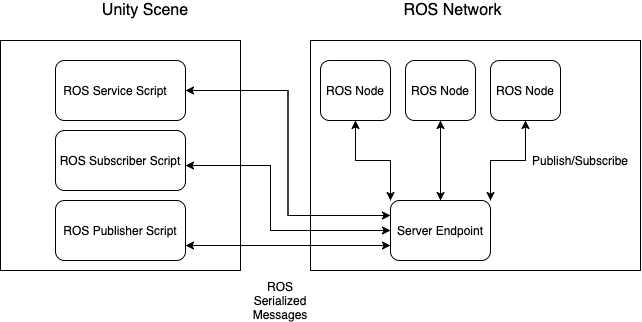
\includegraphics[width=0.75\textwidth]{imagenes/unity_ros.png}
    \caption{\cite{89}}
    \label{Fig:Estructura_Conexion_Unity_ROS}
\end{figure}


\subsubsection{Modo de Control}

Como se especificó, Baxter cuenta con dos brazos -cada uno con 7 grados de libertad- además de poder mover su cabeza en dos ejes. Para poder aprovechar al máximo su movimiento la interfaz de comunicación que posee nos brinda la posibilidad de controlar la posición angular, velocidad y torque de cada una de sus articulaciones para poder situar su efector final en la posición deseada. 

El estado de cada una de las articulaciones puede ser obtenido/establecido mediante mensajes publicados en ROS. Así pues, existen distintos arrays en los que es posible establecer los distintos modos especificados \cite{72}. 

\begin{itemize}
    \item name[i]: id de la i-ésima articulación en los arrays de valores
    \item position[i]: posición de la articulación i-ésima en radianes
    \item velocity[i]: velocidad angular de la articulación i-ésima en rad / s
    \item effort[i]: esfuerzo aplicado en conjunto i-ésima en Nm
\end{itemize}

Los susodichos estados son publicados por robot\_state\_publisher y son actualizados con la información proporcionada por los sensores en cada ciclo. De este modo, la tasa de publicación puede ser establecida mediante la publicación de mensajes de este tópico para lograr una mayor eficiencia o fidelidad.

\section{Entorno de Trabajo con Touch X}

\subsection{Inicialización del Entorno}

Tras inicializar el entorno con Baxter, comenzamos con las pruebas de control del dispositivo háptico y su correcta integración en Unity a través de los plugins y demostraciones disponibles.

\subsubsection{Estudio de la Integración de Touch X y Unity}

Una vez comenzamos la parte del trabajo relativa al control del dispositivo junto a Unity nos topamos con dos principales plugins disponibles en la Asset Store de este último. Los mismos integran funcionalidades y casos de demostración desarrollados en este motor gráfico, haciendo patente que es posible el funcionamiento conjunto de ambas tecnologías.

En primer lugar, procedemos a tratar de conocer su funcionamiento y las llamadas a la API que estos realizan, analizando los scripts que implementan el comportamiento del dispositivo háptico en consecuencia a la simulación. Tras conocer la metodología de trabajo de los mismos, consideramos posible la integración de estos junto a los controladores desarrollados por nuestra parte para el movimiento de Baxter en relación a Touch X.

Entre otras cuestiones, encontramos las mencionadas extensiones están diseñadas para el control de un dispositivo con un volumen y superficie reducidos, extrapolando la aplicación de la fuerza a un solo punto. No obstante esto no es un problema, ya que el feedback que proporcionaremos resulta ser simplemente un vector, por lo que podemos obtener en cada colisión del brazo robótico con los objetos que le rodean todos los puntos de impacto y vectores normales relativos haciendo una sumatoria de las fuerzas resultantes \cite{73,74}.  

Sin embargo, esta metodología de trabajo resulta inviable, ya que el acceso al dispositivo por parte de la susodicha extensión y la metodología de control desarrollada por nuestra parte se torna imposible por errores de exclusión mutua y reserva del dispositivo por parte del primero aparentemente.

Es por ello que decidimos, tras repetidos intentos infructuosos de combinaciones para conseguir lograr la antedicha tarea, desarrollar nuestra propia interpretación de la retroalimentación háptica en consecuencia a la simulación.

\subsection{Metodología de Control}
Asimismo, como se consiguió anteriormente, en primer lugar será necesaria la importación de las funciones implementadas en la citada API, que nos permitirá el acceso a los datos relativos al estado del dispositivo y su control, cuestión que no fue aclarada en la sección que detalla el movimiento de baxter. Para ello haremos uso de los archivos .dll.

\begin{itemize}
    \item DLL: Se denominan bibliotecas de enlace dinámico aquellos archivos compilados cuyo contenido consiste en código ejecutable que se interpreta bajo la demanda de un programa ejecutado en el sistema operativo. 

    Gracias a estos se consigue el empaquetado de información y funciones relativas a un mismo fin reduciendo el espacio necesario para ello, consiguiendo una gran modularización para el acceso por parte de distintas aplicaciones y optimizando la memoria utilizada \cite{75}.
\end{itemize}

Consecuentemente, incluiremos en nuestro proyecto de Unity los archivos del tipo descrito, que se incluyen en el árbol de directorios de instalación de OpenHaptics, para extraer las implementaciones que permiten el acceso a la interfaz de control de Touch X.

\subsubsection{Implementación del Feedback en Colisión}
Como se comentó, en las tareas de mantenimiento que se realizarán en el contexto descrito, será usual la manipulación de objetos. En esta tarea, es relevante conocer la dirección y sentido del impacto que se produce además de la magnitud del mismo para evitar posibles daños a los equipos o las propias instalaciones. Es por ello que la retroalimentación respectiva a los impactos se ha desarrollado de forma en que el usuario pueda sentir levemente los roces o choques leves y que sienta una fuerza bastante más elevada a la hora de tratar de atravesar un objeto.

Detectar que estamos colisionando no es una tarea complicada en Unity, sin embargo, debemos conocer cuál es exactamente la articulación dentro de baxter está colisionando. Para lograr esta tarea haremos que cada una de las articulaciones hijas que componen el brazo notifique su colisión a un script maestro que procesará la información en consecuencia.

Así pues, una vez detectamos el contacto, analizaremos la colisión obteniendo todos los puntos de contacto de la misma para acto seguido calcular el vector de dirección resultante de la suma de todos ellos, obteniendo así la dirección del torque que deberemos establecer en sentido contrario. En este caso, identificaremos si el brazo se encuentra solamente apoyado sobre el plano, estableciendo una fuerza mínima para que pueda sostenerse por sí solo. Además de esto, guardaremos el estado de las articulaciones componentes de Touch X en ese instante para posteriormente conocer cuál es el vector que define la dirección de desplazamiento respecto al instante de colisión.

Asimismo, es una tarea necesaria establecer algunas condiciones para la detección de nuevas colisiones para no confundir los errores de precisión del operario o de las lecturas proporcionadas por Unity y el dispositivo háptico. Es por ello que establecemos distintas consideraciones como no recalcular una nueva colisión si la distancia no supera un cierto umbral establecido a través de sucesivos test en ejecución.

En este momento, como se referenció anteriormente, estableceremos una fuerza de torque creciente dependiendo del desplazamiento que se haga en Touch X, que como sabemos controla a Baxter. De este modo, a través de distintos métodos, determinaremos cuando realmente tratamos de penetrar un objeto y en qué medida pretendemos hacerlo, para establecer una resistencia creciente en el movimiento del dispositivo háptico en esa dirección.

Para ello, establecemos una relación entre los componentes del brazo háptico y el eje al que aportan movimiento, es decir, consideramos el eje de giro de cada articulación para posteriormente realizar una ponderación de la influencia en el desplazamiento en el mismo.

La función elegida para la representación de la fuerza será una exponencial que dependerá de algunas constantes establecidas con el testeo en el proceso de implementación. En concreto definimos una función por partes cuya variable, x, será la cantidad de penetración que se trata de realizar, calculada como la variación entre la posición de las articulaciones al inicio del contacto con un objeto y la actual. Se definen pues $MIN_T = 40$, como el torque mínimo    que utilizaremos y $MAX_T = 1200$, como el máximo a usar.


$$
    f(x)= \left\{ \begin{array}{lcc}
             0 & si  & x < 0.02 \\
            \\ MIN_T + e^{(\ln(MAX_T-MIN_T)/MAX_P)*0.06}*0.7 & si & x > 0.02  \hspace{10pt} y \hspace{10pt} x < 0.06 \\
            \\ MIN_T + e^{(\ln(MAX_T-MIN_T)/MAX_P)*x}*0.7 & si & x > 0.06 \hspace{10pt} y \hspace{10pt} x < 0.1 \\
             \\ MIN_T + e^{(\ln(MAX_T-MIN_T)/MAX_P)*x} & si & x > 0.1\\
             \end{array}
   \right.
$$

Se definen en esta función distintos tramos, establecidos tras la iterativa realización de pruebas. De este modo, la variable $MIN_T$ representará el mínimo torque -establecido como 40 mNm por ser la mínima fuerza necesaria para que el dispositivo pueda sostenerse por sí solo, emulando estar apoyado-. Por el contrario, $MAX_T$ será el valor máximo de torque usado, ya que lo consideramos como suficiente. Así pues, por último, $MAX_P$ se definirá como la máxima penetración establecida para esa articulación, en la cual se alcanza el valor $MAX_T$. En consecuencia, observamos en las figuras \ref{Fig:penetration_02} y \ref{Fig:penetration_03} la evolución del torque para una penetración de 0.2 y 0.3 respectivamente.

\begin{figure}[!htb]
   \begin{minipage}{0.45\textwidth}
     \centering
    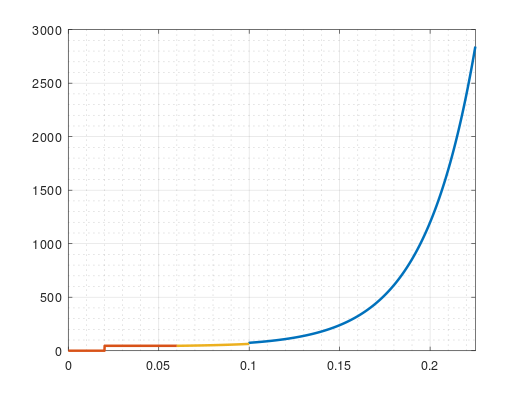
\includegraphics[width=1\textwidth]{imagenes/forceEvolution0.2penetration.png}
    \caption{}
    \label{Fig:penetration_02}
   \end{minipage}\hfill
   \begin{minipage}{0.45\textwidth}
     \centering
    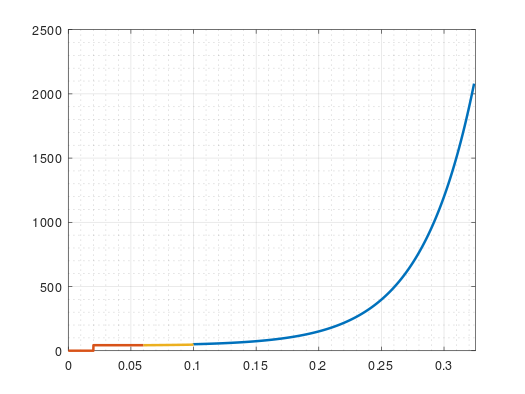
\includegraphics[width=1\textwidth]{imagenes/forceEvolution0.3penetration.png}
    \caption{}
    \label{Fig:penetration_03}
   \end{minipage}
\end{figure}

Gracias a esta y algunos filtros para evitar cambios bruscos, como comparar el nuevo torque que se establecerá con los anteriores valores utilizados, el resultado obtenido se torna agradable al tacto y en general bastante aceptable. 

Además de ello, se toman en consideración algunos casos básicos que se dan en la propia interacción humana con los objetos; como el hecho de solo influir la fuerza normal que nos transmiten los objetos en las articulaciones que preceden a aquella que sufre la colisión,  en el orden que siguen las mismas desde el hombro a la muñeca.

\subsubsection{Implementación de Feedback de Gravedad y Momento de la Fuerza}

Además de conocer las posibles colisiones cuando manipulamos objetos es de gran importancia tener conciencia de la masa asociada a los mismos. En las tareas que conciernen a la teleoperación este factor puede resultar decisivo, ya que a causa de un movimiento brusco o a la carga excesiva de un dispositivo este podría desplomarse. A ese respecto, se ha tratado de realizar una implementación de la gravedad y el torque realistas -contemplando las propiedades físicas exactas de los objetos- a la par que cómoda para el manejo durante un periodo de tiempo moderado.

En este caso, la manera de proceder es bastante intuitiva, ya que consideramos que agarramos un objeto en el momento en que nos acercamos al mismo con el efector final del robot en la simulación y pulsamos el botón que incorpora Touch X en la última de sus articulaciones. No obstante, esta es una mera forma de demostración de las capacidades del dispositivo, ya que Baxter no posee realmente pinzas o manos para prender objetos por defecto en nuestra simulación. Así pues, simplemente sería necesaria la simulación de alguno de los elementos descritos y emular su comportamiento para permitir al robot controlado sujetar elementos de manera realista en la simulación.

Una vez se toma el objeto, se procede al cálculo de las distintas magnitudes intrínsecas en los cuerpos que entran en juego en esta tarea. En este caso utilizamos conceptos básicos de la física newtoniana, como lo son la gravedad, la ley de inercia o la ley fundamental de la dinámica. En consecuencia, cuando el robot agarra un objeto establecemos una fuerza en sentido descendente proporcional al cuerpo prendido, emulando su peso como $\overrightarrow P = m * \overrightarrow g$. En este caso ponderamos las fuerzas entre dos de las articulaciones con feedback en el eje vertical para que la sensación resultante sea una fuerza perpendicular al plano descrito por la superficie en la que se apoya el robot controlado.

Asimismo, procedemos al cálculo del momento de fuerza o torque que sufre el objeto agarrado, despreciando el propio brazo de Baxter para lograr una mayor movilidad y menor cansancio del operario. Por ende, realizamos lecturas en todo momento de la posición del objeto para calcular su velocidad, como $\overrightarrow v =\Delta e/  \Delta t$. Consecuentemente, a partir de la variación de la misma, podemos calcular la aceleración como $ \overrightarrow a = \Delta v/ \Delta t$, para a través del producto escalar de la masa del cuerpo revelar la fuerza en Newtons implícita en el mismo $\overrightarrow F = \Delta a  * m$. Así pues, aplicada la susodicha fuerza a una distancia del punto de aplicación, que será el hombro de Baxter, obtendremos el momento o torque, $\tau = \overrightarrow F*d$ \cite{76}.

Finalmente, como se procedió en la implementación del feedback en el impacto, se establecen distintos métodos para acotar el torque aplicado y evitar movimientos bruscos. Más adelante contemplaremos cómo se lidia con distintos problemas que producen cambios repentinos en el momento aplicado. 

\subsection{API OpenHaptics}
Es necesario hacer uso de su API, como se ha aclarado, para el control del dispositivo háptico. Las interfaces de programación de aplicaciones, se definen como un conjunto de funciones y distintos procedimientos que permiten la conexión y el acceso a los recursos, datos o características de un sistema o aplicación por parte de otro. De este modo, trataremos de controlar Touch X a través de la interfaz que el fabricante nos provee a través de las funciones implementadas en los mencionados archivos .dll que se nos proveen en la instalación del entorno de trabajo del mismo, como se aclaró.

Disponemos de dos maneras de fabricar un nuevo plugin o script controlador haciendo uso de la API que el fabricante del dispositivo nos provee: HDAPI y HLAPI, de las que hablaremos más adelante. La primera obliga al desarrollador a administrar la representación de la fuerza o resistencia que ofrecerá el dispositivo háptico, mientras que HLAPI trata los cálculos de representación háptica basada en primitivas geométricas, transformaciones y propiedades de los materiales proporcionadas por el usuario, lo que resulta en una menor dificultad para el programador; a costa de una ligera pérdida de flexibilidad \cite{77}.

\subsubsection{HDApi}
La interfaz de aplicación HDApi del dispositivo, de la cual hemos hecho uso para la implementación en este estudio, puede ser dividida en dos componentes esenciales principalmente, como lo son el propio dispositivo y el planificador de tareas incorporado. De este modo, la construcción de la interfaz para el acceso al dispositivo permite el soporte de distintos robots con retroalimentación háptica comercializados por 3DSystems.

En este caso, las llamadas a funciones permiten al programador planificar distintas tareas que se ejecutarán en el bucle servidor que se pone a disposición en el momento de uso. De este modo, como se procede en la implementación realizada para este estudio, un programa típico inicializará el dispositivo y el planificador ejecutando a continuación los comandos de realimentación háptica que estime oportunos, para finalmente detener todos los servicios haciendo uso de las llamadas disponible para este fin y cerrar el programa.

Es en la ejecución de los antedichos comandos de realimentación háptica, parte más relevante en el uso del robot, que encontramos algunos aspectos a tener en cuenta en el uso de la interfaz que se nos provee. En primer lugar, será necesario activar explícitamente las capacidades hápticas deseadas a través de las llamadas a la API, entre ellas la realimentación de fuerza. Tras ello, en cada operación de acceso al dispositivo para la consulta o fijación de valores para alguna de sus características será necesario el uso de los denominados como marcos hápticos. De esta manera, los susodichos definen un ámbito o contexto en el cual se garantiza que el estado del dispositivo será consistente y, por ende, todas y cada una de las operaciones que se deseen realizar deberán  ejecutarse dentro de los mismos.

Así pues, cabe destacar que que la programación de las funciones en esta estrategia de control tienen un carácter procedural, de modo que deberemos acceder a los valores, tanto en lectura como en escritura, con el paso de valores por referencia y accediendo a los parámetros deseados a través de códigos hexadecimales definidos en los archivos de implementación \cite{77}.

\subsubsection{HLApi}
HLApi es una interfaz diseñada para facilitar la programación de los dispositivos hápticos soportados basada en patrones de OpenGL para el renderizado gráfico construida en C. Esta permite, como se esbozó anteriormente, la definición de primitivas geométricas, como lo son las líneas, triángulos o puntos junto a propiedades específicas que pueden ir acompañadas de propiedades intrínsecas en los materiales que nos rodean como lo son la rugosidad o una alta fricción. 

De este modo, trabajamos de manera similar a la anteriormente descrita HDApi, teniendo que hacer uso de los comandos disponibles para modificar o consultar las características de los objetos representados. Consecuentemente, el estado de un cuerpo descrito por los algoritmos implementados en el robot incluye información relativa al material del que está hecho, el modo en que se renderiza o las posibles transformaciones que pueda sufrir en su movimiento. Del mismo modo, al igual que en HDApi, es posible consultar el estado de los componentes del dispositivo.

En esta metodología de trabajo, tras el renderizado de las figuras especificadas a la API, es característico el uso del renderizado proxy, que se basa en el uso de un punto que sigue la posición del puntero que describen los efectores finales de dispositivo háptico. Así pues, el citado puntero o proxy se actualizará constantemente pudiendo tocar las figuras representadas en sus caras exteriores, aunque pueden especificarse explícitamente las deseadas. La forma en que el dispositivo tratará de penetrar los modelos y por consiguiente la forma en que se hará la representación de la fuerza, será estirando un resorte virtual entre la posición del dispositivo háptico y la posición del comentado puntero \cite{77}.

\subsection{Torque}
Consideramos necesario en este apartado hacer una breve aclaración acerca de los conceptos físicos implicados en el desarrollo de la implementación que se ha llevado a cabo, para lograr así una mayor comprensión de la totalidad de los conceptos implicados en esta obra. Por consiguiente, expondremos a continuación algunas nociones básicas relativas al campo de la mecánica newtoniana que entran  en juego en la representación virtual de los objetos que nos rodean en lo que a las propiedades táctiles respecta.

La citada teoría mecánica vectorial, formulada por el conocido físico Isaac Newton, se considera una formulación específica de la mecánica clásica en el estudio del desplazamiento de los cuerpos y partículas macroscópicas en un sistema de referencia euclídeo. Por consiguiente, esta da por hecho que se comparte un tiempo por todos los presentes en los eventos de este tipo y asume que los descritos sistemas se desplazan a través de  trayectorias definidas.

De este modo, haciendo uso de las medidas de la variación de la posición, velocidad y aceleración, se designa como momento de una fuerza, o torque respecto a un punto de aplicación, a la magnitud obtenida como el producto vectorial del vector que describe la posición del punto en el que aplicamos la fuerza y aquel que representa la fuerza implícita en el cuerpo. Así pues, congruentemente con este enunciado, podemos representar lo descrito mediante la ecuación dada \cite{78,79}:

$$\overrightarrow M = \overrightarrow {OP} \times \overrightarrow F = \overrightarrow r \times \overrightarrow F$$

Así pues, la interpretación de este concepto en el contexto que describe la aplicación de fuerzas en el contacto con objetos o el desplazamiento de los mismos al ser sujetados por Baxter cobra sentido, ya que esta magnitud física describe la capacidad que una fuerza posee para cambiar la rotación o estado de movimiento del cuerpo al que se aplica la fuerza. De este modo, la fuerza normal que presenta un plano al tratar de realizar un esfuerzo por atravesarlo o la fuerza que un objeto posee en su desplazamiento por el hecho de tener aceleración, teniendo en cuenta el brazo de baxter como punto de aplicación, resulta en el torque que representamos y ofrecemos como retroalimentación al usuario.
